\documentclass{article} % For LaTeX2e
\usepackage[T1]{fontenc} % makes Times available under XeTeX/tectonic; harmless with pdflatex
\usepackage{iclr2027_conference,times}

% Optional math commands from https://github.com/goodfeli/dlbook_notation.
\input{math_commands.tex}

\usepackage{hyperref}
\usepackage{url}
\usepackage{graphicx}
\usepackage{booktabs}
\usepackage{adjustbox}
\usepackage{multirow}
\usepackage{amsmath,amssymb}
\usepackage{xcolor}
\usepackage{enumitem}
\usepackage{bm}
\usepackage{wrapfig}
\usepackage{placeins}
\usepackage{tikz}
\usetikzlibrary{arrows.meta}

\newcommand{\sg}{\operatorname{sg}}
\newcommand{\blow}{b_{\mathrm{low}}}
\newcommand{\eref}{e_{\mathrm{ref}}}
\newcommand{\nfe}{\textsc{nfe}}
\newcommand{\pmsd}[1]{{\scriptsize$\pm$#1}}
\newcommand{\ours}{PaletteDiff}
\newcommand{\gray}[1]{\textcolor{gray}{#1}}

\title{\ours: Native-Resolution Pixel-Art Sprite Generation\\ with Palette-Projected Diffusion}

% Anonymous submission: \iclrfinalcopy stays commented out.
\author{Anonymous authors\\Paper under double-blind review}

\begin{document}

\maketitle

\begin{abstract}
Game sprites of 12--24\,px are among the smallest images people draw on purpose, and their medium is defined by a
handful of flat colours and hard alpha edges. Despite rapid progress in text-to-image generation, existing systems
render such sprites as shrunken illustrations with soft shading and around a hundred colours. We identify two root
causes: the training targets of sprite corpora are dominated by downscaled artwork rather than native pixel art, and
continuous diffusion has no mechanism to express the few-colour structure of the medium. To address these challenges,
we propose \ours{}, a framework for native-resolution sprite generation. First, we introduce \emph{Native-Resolution
Target Rebuilding}, which removes duplicate leakage, forbids aggressive downscaling and adds 15k permissively
licensed sprites, together with a \emph{native evaluation protocol} that scores against real low-resolution pixel art
only. Second, we propose \emph{Palette-Projected Sampling}, a training-free decoding rule that projects the predicted
clean image onto a per-sprite $k$-colour palette during the late denoising steps, so that the remaining steps repair
the quantisation seams. Third, combined with SDEdit-style re-noising, the same rule yields a \emph{Palette Refinement}
module for sprites from generators we did not train. \ours{} lowers FD-DINOv2 at 16\,px from 167.2 to $31.8\pm0.5$;
a per-sprite palette is the decisive ingredient, and imposing it inside the sampler improves on the same quantisation
applied afterwards by a further 18\%. Under the native protocol, \ours{} has the lowest FD among gpt-image-2,
FLUX.2 and SDXL pipelines given the same palette post-process; Palette Refinement improves all three external systems
by 36--41\% while preserving 80\% of their silhouettes.
\end{abstract}

% ================================================================================================================
\begin{figure}[h]
\centering
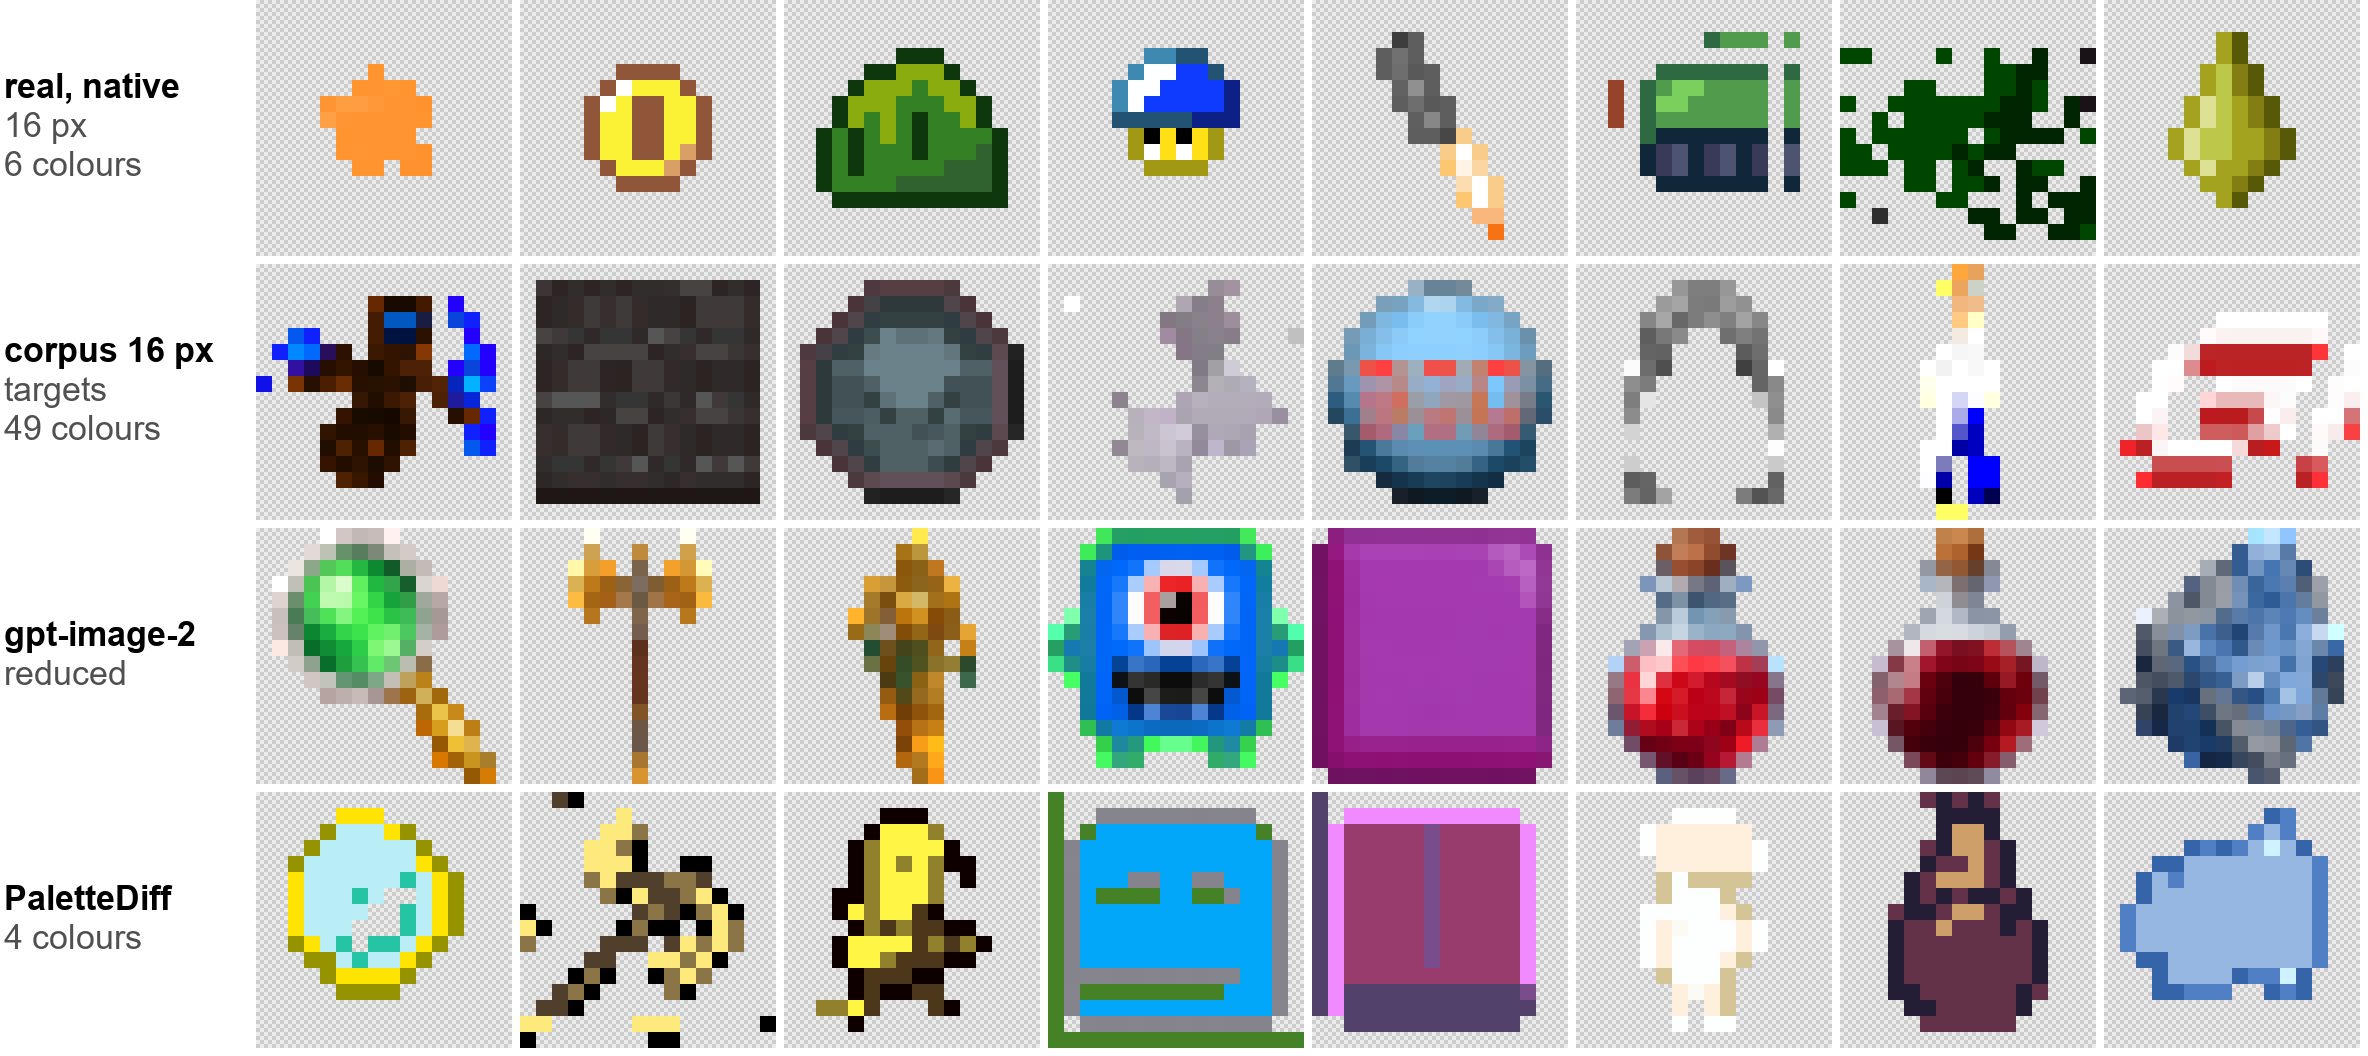
\includegraphics[width=0.92\linewidth]{figures/fig_teaser.png}
\caption{16\,px RGBA sprites, nearest-neighbour magnified. \textbf{Row 1}: real sprites drawn at this size (median six
opaque colours). \textbf{Row 2}: what a conventional sprite corpus feeds into its 16\,px bucket --- 25--64\,px artwork
box-downscaled (median 49 colours). \textbf{Row 3}: gpt-image-2 rendered at 1024\,px and reduced. \textbf{Row 4}:
\ours{} (4 colours), which reproduces the flat colour regions of native pixel art. Colour counts are per-row
medians.}
\label{fig:teaser}
\end{figure}

\section{Introduction}
\label{sec:intro}

Game sprites are among the smallest images anyone draws on purpose: an item, a character or an effect on a 12--24\,px
RGBA canvas, built from hard edges, a handful of flat colour regions and a transparent background, and a staple of 2D
games and procedural content. At these sizes there is no texture in which to hide a mistake: one wrong pixel changes the silhouette, and one blended
colour reads as blur. Recent text-to-image models~\citep{Podell2023,FLUX2} have demonstrated remarkable capability at
high resolution, and the natural recipe is to prompt such a model and shrink its output. The result is recognisable
but it is not a sprite: it keeps the soft shading and the hundred-odd colours of an illustration
(Figure~\ref{fig:teaser}, row 3).

We train a dedicated generator for this medium and identify two primary bottlenecks that hinder tiny-sprite
generation. \textbf{1) Contaminated targets.} A sprite corpus assembled in the standard way --- cutting sheets into
connected components, bucketing by size and downscaling to fill each bucket --- contains little native pixel art: in
ours only 7.1\% of the images are natively 16\,px or smaller, so 92.9\% of what the 16\,px bucket sees is larger art
box-downscaled into it, two thirds of it from 25--64\,px. Exact duplicates additionally leave a pixel-identical twin in training for 16.2\% of
the held-out set. A model fitted to these targets learns soft, fifty-colour blobs, and an evaluation reference drawn
from the same pool rewards exactly that. \textbf{2) Palette mismatch.} Real 16\,px sprites use a median of six opaque
colours and 46\% of their adjacent opaque pixel pairs are exactly equal. A continuous diffusion model in RGB has no
mechanism that snaps a region to a single value: every sampling rule we tested emits around fifty colours and reaches
only 8\% equal neighbours, spending the difference on few-level dither inside regions that should be flat.

To address these challenges, we propose \ours{} (Figure~\ref{fig:overview}). \emph{Native-Resolution Target Rebuilding}
removes duplicate leakage, forbids feeding a sprite to a bucket more than $1.5\times$ below its native size, and adds
14{,}999 permissively licensed sprites, together with a \emph{native protocol} that evaluates against real sprites
drawn at the target size. \emph{Palette-Projected Sampling} (PPS) then projects the predicted clean image onto a
per-sprite $k$-colour palette during the late denoising steps, so the remaining steps repair the quantisation seams;
it is training-free and transfers to a transformer backbone. Combined with SDEdit-style re-noising
\citep{Meng2022sdedit}, the same rule is a \emph{Palette Refinement} module for external generators.

At 16\,px the rebuilt targets move FD-DINOv2 from 167.2 to 117.9, and PPS brings it to $31.8\pm0.5$. Among practitioner
pipelines used zero-shot --- gpt-image-2, FLUX.2 with a pixel-art LoRA and SDXL with Pixel Art XL --- \ours{} has the
lowest native FD even when those systems receive the same palette post-process, and Palette Refinement improves all
three by 36--41\% while preserving 80\% of their silhouettes. Our main contributions are:
\begin{itemize}[leftmargin=1.2em,itemsep=1pt,topsep=2pt]
  \item \textbf{Native-Resolution Target Rebuilding and the native protocol.} We diagnose target contamination and
  duplicate leakage in sprite corpora, and provide a rebuilt corpus and an evaluation protocol grounded in real
  low-resolution pixel art.
  \item \textbf{Palette-Projected Sampling.} A training-free decoding rule that enforces the few-colour structure of
  the medium inside the sampler, transfers to a transformer backbone, and outperforms post-hoc quantisation, a
  corpus-wide palette and de-dithering filters.
  \item \textbf{Palette Refinement.} SDEdit-style re-noising combined with PPS, which transfers the decoding rule to
  generators we did not train, with an explicit dial between preserving the input and matching the medium.
\end{itemize}

\begin{figure}[t]
\centering
\resizebox{0.98\linewidth}{!}{\definecolor{ovA}{RGB}{36,92,160}
\definecolor{ovB}{RGB}{196,86,18}
\definecolor{ovC}{RGB}{28,122,74}
\begin{tikzpicture}[
  font=\sffamily\scriptsize,
  >={Stealth[length=2.2mm]},
  spr/.style={inner sep=0.4pt, draw=black!25, line width=0.35pt, fill=white},
  box/.style={draw=#1!75!black, fill=#1!12, rounded corners=2pt, align=center,
              inner sep=2.4pt, line width=0.65pt, font=\sffamily\scriptsize},
  note/.style={align=center, font=\sffamily\tiny, text=black!62},
  arr/.style={->, line width=0.85pt, draw=#1!80!black},
]
\def\S{1.18cm}
\newcommand{\badge}[2]{%
  \tikz[baseline=-0.6ex]\node[circle, fill=white, text=#1, font=\sffamily\bfseries\scriptsize,
    inner sep=0.9pt, minimum size=0.32cm]{#2};}
\newcommand{\panel}[6]{% x0 y0 x1 y1 colour title
  \fill[#5!7, rounded corners=3.5pt] (#1,#2) rectangle (#3,#4);
  \draw[#5!55, rounded corners=3.5pt, line width=0.7pt] (#1,#2) rectangle (#3,#4);
  \fill[#5, rounded corners=3.5pt] (#1,#4-0.42) rectangle (#3,#4);
  \fill[#5] (#1,#4-0.42) rectangle (#3,#4-0.18);
  \node[anchor=west, text=white, font=\sffamily\bfseries\scriptsize] at (#1+0.10,#4-0.21) {#6};}

% ── 1 ────────────────────────────────────────────────────────────────
\panel{0.00}{0.00}{7.55}{3.55}{ovA}{\badge{ovA}{1}\;Native-Resolution Target Rebuilding}
\node[spr] (d1) at (0.92,2.15) {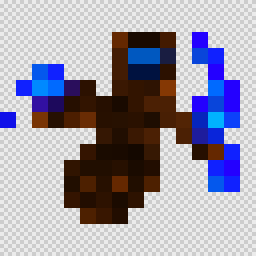
\includegraphics[width=\S]{figures/ov/down.png}};
\node[spr] (d2) at (0.92,0.85) {
\includegraphics[width=\S]{figures/ov/down2.png}};
\node[note, text=ovA!50!black] at (0.92,2.88) {49 colours};
\node[note, rotate=90, text=ovA!45!black] at (0.16,1.50) {downscaled targets};

\node[box=ovA, text width=2.38cm, anchor=west] (c1) at (1.82,2.55)
  {\textbf{dedup} --- no train/test leakage};
\node[box=ovA, text width=2.38cm, anchor=west] (c2) at (1.82,1.55)
  {\textbf{bucket} --- shrink at most $1.5\times$};
\node[box=ovA, text width=2.38cm, anchor=west] (c3) at (1.82,0.55)
  {\textbf{+15k} licensed sprites, 40\% native $\le$24\,px};
\draw[ovA!65, line width=0.7pt] (1.82,0.55) -- (1.82,2.55);
\draw[arr=ovA] (1.55,1.50) -- (1.80,1.50);
\draw[arr=ovA] (4.28,1.50) -- (4.55,1.50);

\node[spr] (n1) at (5.22,2.15) {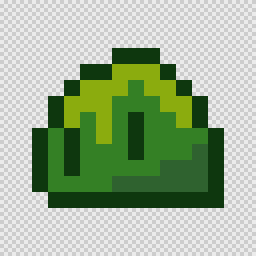
\includegraphics[width=\S]{figures/ov/native.png}};
\node[spr] (n2) at (5.22,0.85) {
\includegraphics[width=\S]{figures/ov/native2.png}};
\node[note, text=ovA!50!black] at (5.22,2.88) {6 colours, native};
\node[box=ovA, text width=1.55cm, font=\sffamily\tiny] at (6.72,1.50)
  {\textbf{native protocol}\\[1pt] FD vs.\ sprites drawn at $\le R$\,px};

% ── 3 ────────────────────────────────────────────────────────────────
\panel{7.70}{0.00}{13.95}{3.55}{ovC}{\badge{ovC}{3}\;Palette Refinement}
\node[spr] at (8.45,2.15) {
\includegraphics[width=\S]{figures/ov/ext.png}};
\node[spr] at (8.45,0.85) {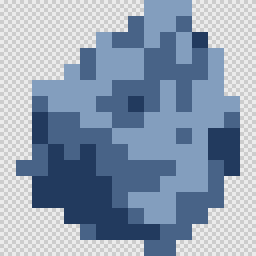
\includegraphics[width=\S]{figures/ov/ext2.png}};
\node[note] at (8.45,2.88) {external sprite};
\node[box=ovC, text width=1.22cm] (rn) at (10.00,1.50) {\textbf{re-noise}\\to $\sigma$\\[-1pt]{\tiny SDEdit}};
\node[box=ovB, text width=1.22cm] (dn) at (11.50,1.50) {\textbf{denoise}\\with PPS\\[-1pt]{\tiny panel 2}};
\node[spr] at (13.10,2.15) {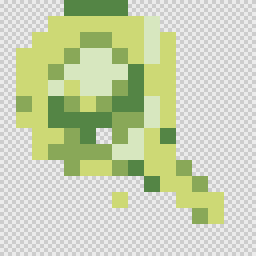
\includegraphics[width=\S]{figures/ov/refined.png}};
\node[spr] at (13.10,0.85) {
\includegraphics[width=\S]{figures/ov/refined2.png}};
\node[note] at (13.10,2.88) {refined sprite};
\draw[arr=ovC] (9.10,1.50) -- (rn.west);
\draw[arr=ovC] (rn.east) -- (dn.west);
\draw[arr=ovC] (dn.east) -- (12.48,1.50);
\node[note, text=ovC!55!black] at (10.75,0.42) {$\sigma$ keeps layout, PPS repaints the medium};

% ── 2 ────────────────────────────────────────────────────────────────
\panel{0.00}{-3.55}{13.95}{-0.12}{ovB}{\badge{ovB}{2}\;Palette-Projected Sampling (PPS)}
\node[anchor=east, text=white, font=\sffamily\tiny] at (13.82,-0.33)
  {training-free $\cdot$ no extra NFEs $\cdot$ UNet or transformer};

\def\y{-1.85}
\node[spr] (xt) at (0.85,\y) {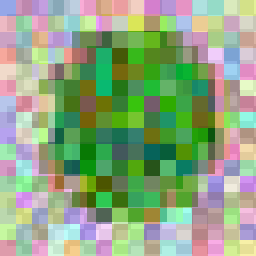
\includegraphics[width=\S]{figures/ov/xt.png}};
\node[note] at (0.85,\y+0.78) {noisy $x_t$};

\node[box=ovB, text width=1.85cm, minimum height=1.05cm] (un) at (2.95,\y)
  {\textbf{denoiser}\\$\epsilon_\theta(x_t,t,c,b)$\\[-1pt]{\tiny + ICG}};
\draw[arr=ovB] (xt.east) -- (un.west);

\node[spr] (x0) at (5.05,\y) {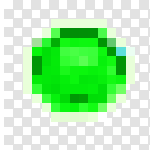
\includegraphics[width=\S]{figures/ov/dither.png}};
\node[note] at (5.05,\y-0.88) {$\hat x_0$: $\sim$50 colours, dither};
\draw[arr=ovB] (un.east) -- (x0.west);

\node[box=ovB, fill=ovB!28, text width=2.05cm, minimum height=1.05cm] (pi) at (7.20,\y)
  {\textbf{project} $\Pi_k(\hat x_0)$\\per-sprite $k$-means\\on opaque pixels};
\draw[arr=ovB] (x0.east) -- (pi.west);

\node[spr] (xp) at (9.35,\y) {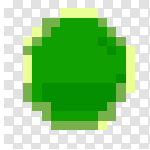
\includegraphics[width=\S]{figures/ov/pal.png}};
\node[note] at (9.35,\y-0.88) {$\hat x_0^{\mathrm{pal}}$: $k$ flat colours};
\draw[arr=ovB] (pi.east) -- (xp.west);

\node[box=ovB, text width=1.55cm, minimum height=1.05cm] (ep) at (11.35,\y)
  {\textbf{re-derive} $\tilde\epsilon$\\Eq.~(\ref{eq:palette})\\and step};
\draw[arr=ovB] (xp.east) -- (ep.west);

\node[spr] (out) at (13.15,\y) {
\includegraphics[width=\S]{figures/ov/pal2.png}};
\node[note] at (13.15,\y+0.78) {final sprite};
\draw[arr=ovB] (ep.east) -- (out.west);

\draw[arr=ovB, dashed, rounded corners=3pt]
  (ep.south) -- (11.35,-3.22) -- (0.85,-3.22) -- (xt.south);
\node[note, fill=ovB!8, inner sep=1.5pt, text=ovB!65!black] at (6.10,-3.22)
  {later steps see the quantised state and \textbf{repair its seams}\quad($t/T\le f$)};
\end{tikzpicture}
}
\caption{Overview of \ours{}. \textbf{(1)}~Rebuild the targets and score only against sprites drawn at the canvas size.
\textbf{(2)}~Project $\hat x_0$ onto a per-sprite $k$-colour palette in the late steps; later steps repair the seams.
\textbf{(3)}~Re-noise an external sprite and denoise it with (2) to keep its layout while matching the medium.}
\label{fig:overview}
\end{figure}
\FloatBarrier

% ================================================================================================================
\section{Related work}
\label{sec:related}

\paragraph{Pixel art.}
Most work on pixel art converts an existing image rather than generating one: joint palette-and-pixel optimisation
\citep{Gerstner2012}, contrast-aware downscaling \citep[PixelOE;][]{PixelOE2024} and learned pixelization
\citep{Han2018,Wu2022}. Generative approaches include GANs for character sprites \citep{Coutinho2022}, pose-conditioned
sprite sheets \citep{SpriteSheetDiffusion2024}, a palette-conditioned DDPM \citep{PixDiffPIG}, SD-$\pi$XL, which
optimises one image by score distillation from SDXL \citep{Binninger2024}, and community LoRAs on large models
\citep{PixelArtXL,PixelArtLoRAFlux}. \ours{} estimates the palette from the model's own prediction rather than conditioning on it, and generates a sprite
in one sampling pass rather than hours of score distillation.

\paragraph{Guidance for diffusion models.}
Classifier-free guidance \citep{HoSalimans2022} and its variants
\citep{Kynkaanniemi2024,Sadat2024apg,Sadat2025fdg,Sadat2024cads,Chung2024} extrapolate away from an unconditional
prediction; other rules use a weaker model \citep{Karras2024}, perturbed attention \citep{Ahn2024,Hong2023,Hong2024},
a degraded \citep{CDG2026} or a random condition \citep[ICG;][]{Sadat2024icg}. We adopt ICG and show that it composes
with palette projection.

\paragraph{Constraints inside the sampler.}
Projecting the predicted $\hat x_0$ at each step is a standard device for imposing hard constraints on diffusion models,
from plug-and-play priors to inverse-problem solvers \citep{Venkatakrishnan2013,Chung2023dps}; discrete-state
formulations impose quantisation by construction \citep{Austin2021,Gu2022vqdiffusion}. PPS applies this device to the
property that defines pixel art, with a palette estimated on the fly, and keeps the continuous denoiser and its training
unchanged.

\paragraph{Reference sets in generative evaluation.}
FID is known to be sensitive to the feature extractor and preprocessing \citep{Heusel2017,Parmar2022,Stein2023}, and
duplicate contamination affects many image corpora \citep{Barz2020,Webster2023,Torralba2011}. Following
\citet{Stein2023}, we use DINOv2 features \citep{Oquab2023}; our native protocol additionally specifies \emph{which}
real images form the reference, which for tiny sprites turns out to determine the ranking of methods.

% ================================================================================================================
\section{Method}
\label{sec:method}

\subsection{Native-Resolution Target Rebuilding}
\label{sec:data}

\paragraph{Diagnosis.}
Our starting corpus contains 37{,}489 unique sprites cut from OpenGameArt \citep{OpenGameArt} sheets, together with the
Kenney and Liberated Pixel Cup packs. Only 2{,}675 (7.1\%) are natively at most 16\,px and 12{,}516 at most 24\,px; the
remaining two thirds are 25--64\,px artwork that a bucketed training pipeline box-downsamples into the low-resolution
buckets. Downsampling averages
neighbouring pixels, so these targets carry a median of 49 colours against six for sprites drawn at 16\,px
(Figure~\ref{fig:teaser}, rows 1--2). Only 4.6\% of the corpus is integer-upscaled pixel art that could be restored by
dividing by its block size. Hashing every sprite by its exact
pixel content further reveals 4{,}888 duplicate copies; because a held-out set defined by file path cannot see that two
paths hold the same image, 16.2\% of the 3{,}000 held-out evaluation sprites have a pixel-identical twin in training.

\paragraph{Rebuilt targets.}
We (i) drop every duplicate copy and every copy of a held-out sprite; (ii) allow a sprite to feed a bucket only if it is
at most $1.5\times$ larger than that bucket, so that a 64\,px illustration can no longer become a 16\,px target; and
(iii) add 14{,}999 sprites cut from three permissively licensed OpenGameArt collections (CC-BY-4.0, CC-BY-SA-3.0,
OGA-BY-3.0), of which 1{,}726 are natively at most 16\,px and 6{,}028 at most 24\,px, filtered for fonts, UI and
near-identical animation frames and captioned with a vision--language model (13{,}987 usable captions, 99.6\%
distinct). Every added sprite keeps its source and licence in a manifest. The
rebuilt corpus has 86{,}290 training rows and 65\% more natively $\le 16$\,px sprites than before
(Appendix~\ref{app:data}).

\paragraph{Native protocol.}
The reference at resolution $R$ is drawn only from real sprites whose native size is at most $R$, so no downscaling
ever touches it: the natively $\le R$ pool of the original corpus is split in half with a fixed seed into a reference
and a disjoint floor set (at 16\,px: 1{,}337 and 1{,}338 images, real-vs-real floor 4.47). The reference describes the
target distribution and is drawn from the same pool as the training data, which it is not removed from; to measure generalisation without any
overlap, we additionally evaluate on a \emph{training-excluded native set} of held-out sprites that are natively
$\le 16$\,px and were removed from training (Section~\ref{sec:analysis}). We contrast the native reference with the
\emph{biased} reference obtained by sampling the whole corpus, of which 92.9\% is downscaled at 16\,px.

\subsection{Resolution-bucketed sprite diffusion}
\label{sec:model}

We generate RGBA sprites on an $R\times R$ canvas, $R\in\{12,16,20,24\}$, from a caption $c$. The denoiser
$\epsilon_\theta(x_t,t,c,b)$ is a 72.5M-parameter UNet that operates directly on the four-channel image. Text enters
through cross-attention to a frozen CLIP ViT-B/32 text encoder \citep{Radford2021}, and the resolution bucket
$b\in\{12,16,20,24,32,48,64\}$ enters as a class embedding added to the timestep embedding. We train with the
$\epsilon$-objective \citep{Ho2020} on a cosine schedule with $T=1000$ and sample with 100 ancestral DDPM steps. The
design is deliberately minimal, so that the gains we report can be attributed to the targets and the decoding rule;
Section~\ref{sec:ablation} shows that they transfer unchanged to a transformer backbone.

\paragraph{Guidance.}
All guidance rules combine the conditional prediction with a reference on the same state,
$\tilde e = \eref + w\,(\epsilon_\theta(x_t,t,c,b_R) - \eref)$. We use independent-condition guidance
\citep[ICG;][]{Sadat2024icg}, in which the reference replaces the caption embedding by Gaussian noise with matched
standard deviation, redrawn at every step. ICG needs no unconditional training, improves native FD over CFG 1.5 by
30.8, and composes with palette projection.

\subsection{Palette-Projected Sampling}
\label{sec:palette}

A sprite is defined as much by how few colours it uses as by its shape. PPS enforces this property on the model's own
belief. At every step with $t/T\le f$ we form the current clean-image estimate
$\hat x_0 = (x_t - \sqrt{1-\bar\alpha_t}\,\tilde e)/\sqrt{\bar\alpha_t}$, cluster its \emph{opaque} RGB pixels into $k$
groups with a batched $k$-means (8 iterations, deterministic initialisation at evenly spaced luminance quantiles),
replace every pixel by its centroid, leave transparent pixels and the alpha channel untouched, and map the result back
to a noise prediction:
\begin{equation}
  \hat x_0^{\text{pal}} = \Pi_k(\hat x_0), \qquad
  \tilde e \;\leftarrow\; \bigl(x_t - \sqrt{\bar\alpha_t}\,\hat x_0^{\text{pal}}\bigr) / \sqrt{1-\bar\alpha_t},
  \label{eq:palette}
\end{equation}
before taking the scheduler step. The projection is a hard constraint on the model's belief rather than a
post-process: the steps that follow see the quantised state and repair the seams it creates
(Figure~\ref{fig:palette}), which is why PPS clearly outperforms quantising the finished image
(Section~\ref{sec:ablation}). The palette is estimated per sprite, so each sprite keeps its own colours. PPS adds no
network evaluations, since 8 $k$-means iterations over at most 576 pixels are negligible next to a UNet pass, and it
requires no retraining. A pixel counts as opaque when its predicted alpha exceeds 0.5, the same threshold used to
binarise alpha in the data. We use $f=0.5$ throughout.

\begin{figure}[t]
\centering

\includegraphics[width=0.64\linewidth]{figures/fig_palette.png}
\caption{Palette-Projected Sampling at 16\,px, same prompts and seed; panel titles give the guidance weight and native
FD of each row. Without projection (top), flat regions carry a few levels of dither. Projecting the predicted
$\hat x_0$ onto six (middle) or four (bottom) colours during the late steps removes it, and the remaining denoising
steps repair the seams, producing clean flat regions and crisp outlines.}
\label{fig:palette}
\end{figure}

\subsection{Palette Refinement of external sprites}
\label{sec:refinemethod}

Because PPS acts on the sampler state, it can be applied to an image the model did not generate. Following SDEdit
\citep{Meng2022sdedit}, we re-noise a sprite produced by an external pipeline and reduced to the canvas to a fraction
$\sigma$ of the schedule, and denoise it with \ours{} under ICG and PPS. The parameter $\sigma$ is an explicit dial:
small values preserve the input, and $\sigma=1$ discards it and recovers generation from noise, which we use only as a
consistency check. This combines a large generator's layout and subject with a sprite drawn in the grammar of the
medium.

% ================================================================================================================
\section{Experiments}
\label{sec:exp}

\subsection{Experimental setup}
\label{sec:protocol}

\paragraph{Evaluation.}
For every configuration we draw one sample for each of 3{,}000 held-out captions, the recaptions of 3{,}000 held-out
sprites. Our primary metric is the Fréchet distance of DINOv2-small CLS features \citep{Oquab2023,Stein2023} (FD, lower
is better) under the native protocol; images are composited on white and nearest-neighbour upsampled to 224\,px. We
also report CLIP ViT-B/32 image--text similarity ($100\cos$) and retrieval R@1 of the own caption among 100. The
seed-to-seed standard deviation of our headline configuration is 0.49 over three seeds; single-seed numbers therefore
differ from the three-seed mean by a few tenths (e.g.\ 31.6 for seed 0). The palette size $k$, the start $f$ and the
guidance weight $w$ were selected on the evaluation FD; at 16\,px we verify that the selection of $k$ transfers between
disjoint halves of the captions (Section~\ref{sec:ablation}).

\paragraph{Baselines.}
We compare against three publicly available text-to-sprite pipelines: gpt-image-2 \citep{GPTImage2}, FLUX.2-klein-4B \citep{FLUX2} with a
pixel-art LoRA \citep{PixelArtLoRAFlux}, and SDXL \citep{Podell2023} with Pixel Art XL \citep{PixelArtXL}. Each generates
at its native size and is reduced to the sprite canvas by the same cutout and downsampling code we use for real data.
At 16\,px, box downscaling is the strongest conversion we found: on gpt-image-2, measured against the corpus-sample
reference, PixelOE \citep{PixelOE2024} and learned pixelization \citep{Wu2022} give 146.3 and 155.2 against 82.2 for
box downscaling (Appendix~\ref{app:externalfig}). Every baseline additionally receives the same $k$-colour palette post-process that PPS
applies inside our sampler. SD-$\pi$XL \citep{Binninger2024} requires about 8 GPU-hours per sprite and is therefore not
evaluated at scale.

\paragraph{Implementation details.}
The main model is trained from scratch for 80k steps with AdamW at a constant learning rate of $5\cdot10^{-5}$, EMA
0.999 and 10\% caption dropout. We use ICG with $w=2$ and PPS with $k=4$ at 16\,px unless stated otherwise;
Appendix~\ref{app:details} lists all hyperparameters.

\subsection{Comparison with state-of-the-art systems}
\label{sec:external}

\begin{table}[t]
\caption{Comparison with external systems, 200 held-out captions (external generation is costly), native FD
$\downarrow$. FD at $n{=}200$ is biased upwards relative to $n{=}3000$ (ours: 53.1 vs.\ 31.8), identically for every
row. Every baseline receives the same $k$-colour post-process ($k=4/8/6$ at 16/20/24\,px) that \ours{} applies inside
its sampler. Ours at 16\,px is the mean of three seeds (50.8 / 52.9 / 55.4), 20 and 24\,px are single seeds. The gray
row, real held-out sprites of the original mixed-provenance corpus with the same post-process, is the ground truth of
the conventional protocol and is shown for reference.}
\label{tab:external}
\centering
\small
\begin{tabular}{@{}lccc@{}}
\toprule
Method & 16\,px & 20\,px & 24\,px \\
\midrule
SDXL + Pixel Art XL LoRA          & 244.2 & 526.3 & 527.2 \\
FLUX.2-klein + pixel-art LoRA     & 150.1 & 473.9 & 472.4 \\
gpt-image-2 + downscale           & 134.4 & 448.6 & 478.0 \\
\textbf{\ours{} (ours)}           & \textbf{53.1 \pmsd{2.3}} & \textbf{152.5} & \textbf{192.2} \\
\midrule
\gray{Real sprites (mixed provenance)} & \gray{77.0} & \gray{165.5} & \gray{150.7} \\
\bottomrule
\end{tabular}
\end{table}

\begin{figure}[t]
\centering
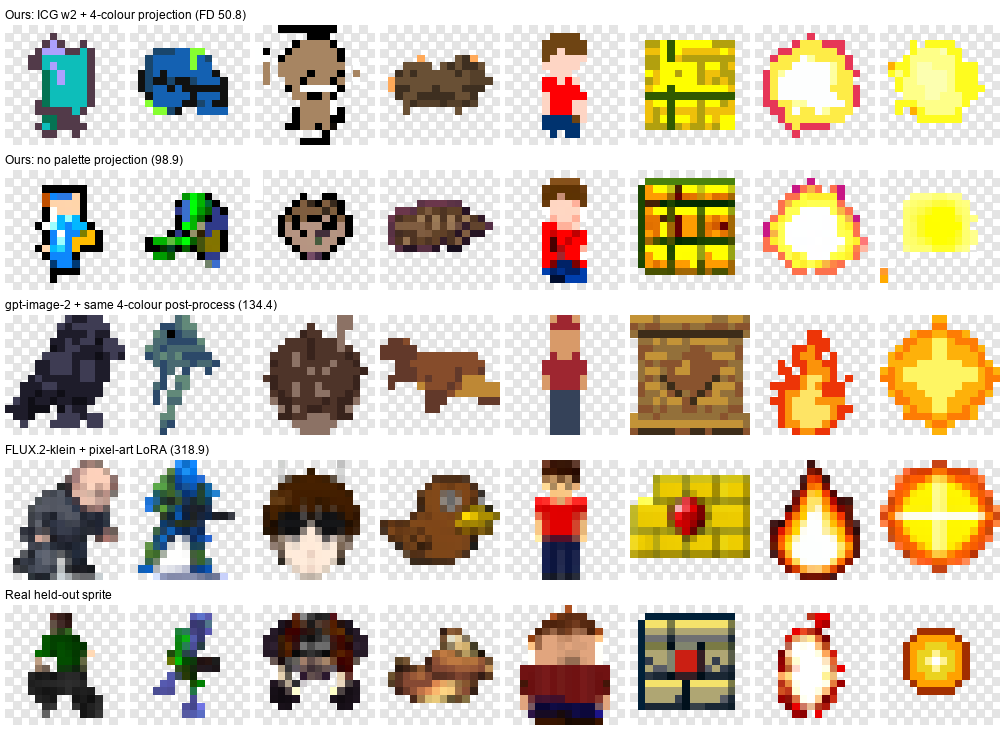
\includegraphics[width=0.78\linewidth]{figures/fig_external.png}
\caption{Qualitative comparison at 16\,px on eight held-out captions. Rows: \ours{}; \ours{} without palette projection;
gpt-image-2 generated at 1024\,px, reduced and given the same four-colour post-process; FLUX.2-klein with a pixel-art
LoRA, reduced \emph{without} the post-process (Table~\ref{tab:external} reports it with the post-process, 150.1); the
real held-out sprite. The FLUX row is unquantised so the residual illustration look is visible; the table is the
fair, post-processed comparison. Numbers in the row titles are single-seed native FD ($n=200$).}
\label{fig:external}
\end{figure}

Table~\ref{tab:external} and Figure~\ref{fig:external} compare \ours{}, a specialist trained on sprites, with
general-purpose generators used zero-shot, which is how practitioners obtain sprites today. \ours{} achieves the
lowest native FD at every resolution, 2.5--4.6$\times$ below every zero-shot baseline even
though those baselines receive the same palette post-process; without it, gpt-image-2, FLUX.2 and SDXL score 284.4, 318.9
and 436.4 at 16\,px. The post-process itself does not explain the gap: real mixed-provenance sprites with the same
four-colour quantisation score 77.0, so quantisation alone does not reach our 53.1. That row is dominated by
downscaled artwork (Section~\ref{sec:data}); against it, \ours{} is better at 16 and 20\,px and behind at 24\,px. Qualitatively, the external systems
draw miniature paintings with soft gradients and anti-aliased outlines, while \ours{} produces the flat regions of
sprites authored at this size.

\subsection{Ablation study}
\label{sec:ablation}

\begin{table}[t]
\caption{Ablation of the components of \ours{}, 16\,px, 3{,}000 held-out captions: native FD $\downarrow$, and CLIP
$100\cos$ / retrieval R@1 where measured (real held-out sprites: 27.66 / 22.6\%). ``Post-hoc'' quantises the finished
samples to the same palette size.}
\label{tab:main16}
\centering
\small
\begin{tabular}{@{}lllcc@{}}
\toprule
Targets & Guidance & Palette & Native FD $\downarrow$ & CLIP / R@1 \\
\midrule
original          & CFG 1.5   & ---                & 167.2 & -- \\
w/o new sprites   & CFG 1.5   & ---                & 123.1 & -- \\
rebuilt           & CFG 1.5   & ---                & 117.9 & -- \\
rebuilt           & ICG 2     & ---                & 87.1  & 27.60 / 22.8\% \\
\midrule
original          & ICG 2     & PPS, $k{=}4$       & 42.9  & -- \\
rebuilt           & CFG 1.5   & PPS, $k{=}4$       & 58.4  & -- \\
rebuilt           & ICG 1.5   & post-hoc, $k{=}4$  & 41.6  & -- \\
rebuilt           & ICG 1.5   & PPS, $k{=}4$       & 34.1  & -- \\
rebuilt           & ICG 2     & PPS, $k{=}6$       & 36.9  & 27.38 / 22.0\% \\
\textbf{rebuilt}  & \textbf{ICG 2} & \textbf{PPS, $\bm{k{=}4}$} & \textbf{31.8 \pmsd{0.49}} & 27.07 / 19.2\% \\
\bottomrule
\end{tabular}
\end{table}

\paragraph{Effect of each component.}
Table~\ref{tab:main16} shows that every component contributes. Rebuilding the targets alone improves FD from 167.2 to
117.9 without touching the sampler, and the new sprites account for a further 5.2 on top of the bucket policy. ICG
brings it to 87.1, and PPS to $31.8\pm0.5$, a step of 55.3. The components are complementary: PPS on the original
targets reaches 42.9 and PPS with plain CFG reaches 58.4, while the full combination reaches 31.8.

\paragraph{In-sampler projection vs.\ post-processing.}
At ICG 1.5 (87.2 without a palette), quantising the finished samples to four colours already reaches 41.6, which
identifies the per-sprite palette as the decisive property of the medium. Imposing the same palette inside the sampler
reaches 34.1, a further 18\%: the steps that follow the projection repair the seams that quantisation introduces, which
a post-process cannot do.

\paragraph{Is it the per-sprite palette?}
Two controls replace $\Pi_k$ at exactly the same steps. Projecting onto \emph{one} four-colour palette shared by every
sprite, learned by $k$-means over the reference set, gives 120.1; a $3\times3$ median filter, which removes the same
dither without imposing a palette, gives 112.2. Both are far from PPS (31.6 with the same seed), confirming that the gain
comes from each sprite's own small palette rather than from fewer colours or smoothing alone.

\paragraph{Palette size and schedule.}
Sweeping $k$ at 16\,px gives 38.1 / 31.8 / 33.7 / 36.9 / 50.6 for $k=3/4/5/6/8$: every setting improves over no
projection (87.1) by a wide margin. The choice of $k$ transfers across a validation split: selecting on one half of the
captions picks $k=4$, which is also best on the disjoint half. At $k=6$ the samples reproduce the colour statistics of
real sprites (six colours and 43\% equal neighbours, vs.\ six and 46\%) and are as retrievable from their captions as
the real sprites (R@1 22.0\% vs.\ 22.6\%); $k=4$ trades 2.8 points of retrieval for the best FD, and we recommend
$k=6$ when prompt fidelity matters most. PPS is also robust to its start point: single-seed runs give 31.4 and 31.6 at
$f=0.4$ and $0.5$ (within seed noise), and running it for the entire schedule still gives 33.7.

\paragraph{Generality across backbones.}
We replace the UNet with a 69.7M-parameter transformer (PixArt-style adaptive norm; \citealt{Chen2023pixart}), keeping corpus, schedule, sampler
and evaluation unchanged, and compare the two at 20k steps with two seeds each. Under plain CFG the transformer trails
by 36.5 FD (185.6 vs.\ 149.1); with ICG and PPS the transformer reaches 42.4 and the UNet 43.1 (seed spread at most
0.4), bringing two backbones that differ markedly under CFG to the same level.

\begin{table}[t]
\centering
\begin{minipage}[t]{0.49\linewidth}
\centering
\caption{Other resolutions, native FD $\downarrow$ (ICG $w{=}2$). Ours: three seeds at 12--24\,px.}
\label{tab:res}
\small
\begin{tabular}{@{}lccc@{}}
\toprule
Res. & w/o PPS & \ours{} ($k$) & Gain \\
\midrule
12\,px & 155.7 & \textbf{143.2 \pmsd{0.8}} (8) & 8\% \\
16\,px & 87.1  & \textbf{31.8 \pmsd{0.5}} (4) & 63\% \\
20\,px & 117.0 & \textbf{96.5 \pmsd{0.9}} (8) & 18\% \\
24\,px & 186.8 & \textbf{123.6 \pmsd{0.5}} (6) & 34\% \\
32\,px & 97.1  & \textbf{74.5} (8) & 23\% \\
\bottomrule
\end{tabular}
\end{minipage}\hfill
\begin{minipage}[t]{0.49\linewidth}
\centering
\caption{Palette Refinement of external sprites, 16\,px, native FD $\downarrow$ and silhouette IoU with the input at
$\sigma{=}0.6$ (a fresh sample scores 0.46--0.53).}
\label{tab:refine}
\small
\begin{tabular}{@{}lcccc@{}}
\toprule
System & input & $\sigma{=}0.4$ & $\sigma{=}0.6$ & IoU \\
\midrule
gpt-image-2  & 134.4 & 115.9 & \textbf{86.5}  & 0.79 \\
FLUX.2       & 150.1 & 116.1 & \textbf{88.2}  & 0.80 \\
SDXL         & 244.2 & 197.2 & \textbf{155.0} & 0.81 \\
\bottomrule
\end{tabular}
\end{minipage}
\end{table}

\paragraph{Other resolutions.}
Table~\ref{tab:res} shows that \ours{} improves native FD at every canvas size from 12 to 32\,px. Absolute values are
not comparable across rows: each resolution has its own native reference (half of the natively $\le R$\,px pool, e.g.\
355 sprites at 12\,px) and its own floor. The recipe is not specific to our target range: at 32\,px PPS improves ICG
from 97.1 to 74.5, and CFG scores 139.2.

\subsection{Palette Refinement of external generators}
\label{sec:refine}

Table~\ref{tab:refine} applies Palette Refinement to the three external pipelines. We measure retention as the IoU of
the alpha mask with the input sprite, since DINOv2 similarity is saturated at this size. At $\sigma=0.6$, native FD
improves by 36--41\% for all three systems while the mask IoU stays near 0.8, well above the 0.46--0.53 of a freshly
generated sprite for the same caption. On gpt-image-2 the same $\sigma$ takes native FD from 448.6 to 265.7 at 20\,px
and from 478.0 to 299.0 at 24\,px (IoU 0.84 / 0.88). Sweeping $\sigma$ is monotone (134.4 / 115.9 / 86.5 / 53.6 at
$\sigma=0 / 0.4 / 0.6 / 1$); $\sigma=1$ recovers our own samples (53.6 vs.\ 53.1). At $\sigma=0.6$, refinement retains
most of the large generator's caption retrieval (18.5\% vs.\ 22.0\%) while moving its style towards the medium
(Figure~\ref{fig:refine}).

\begin{figure}[t]
\centering
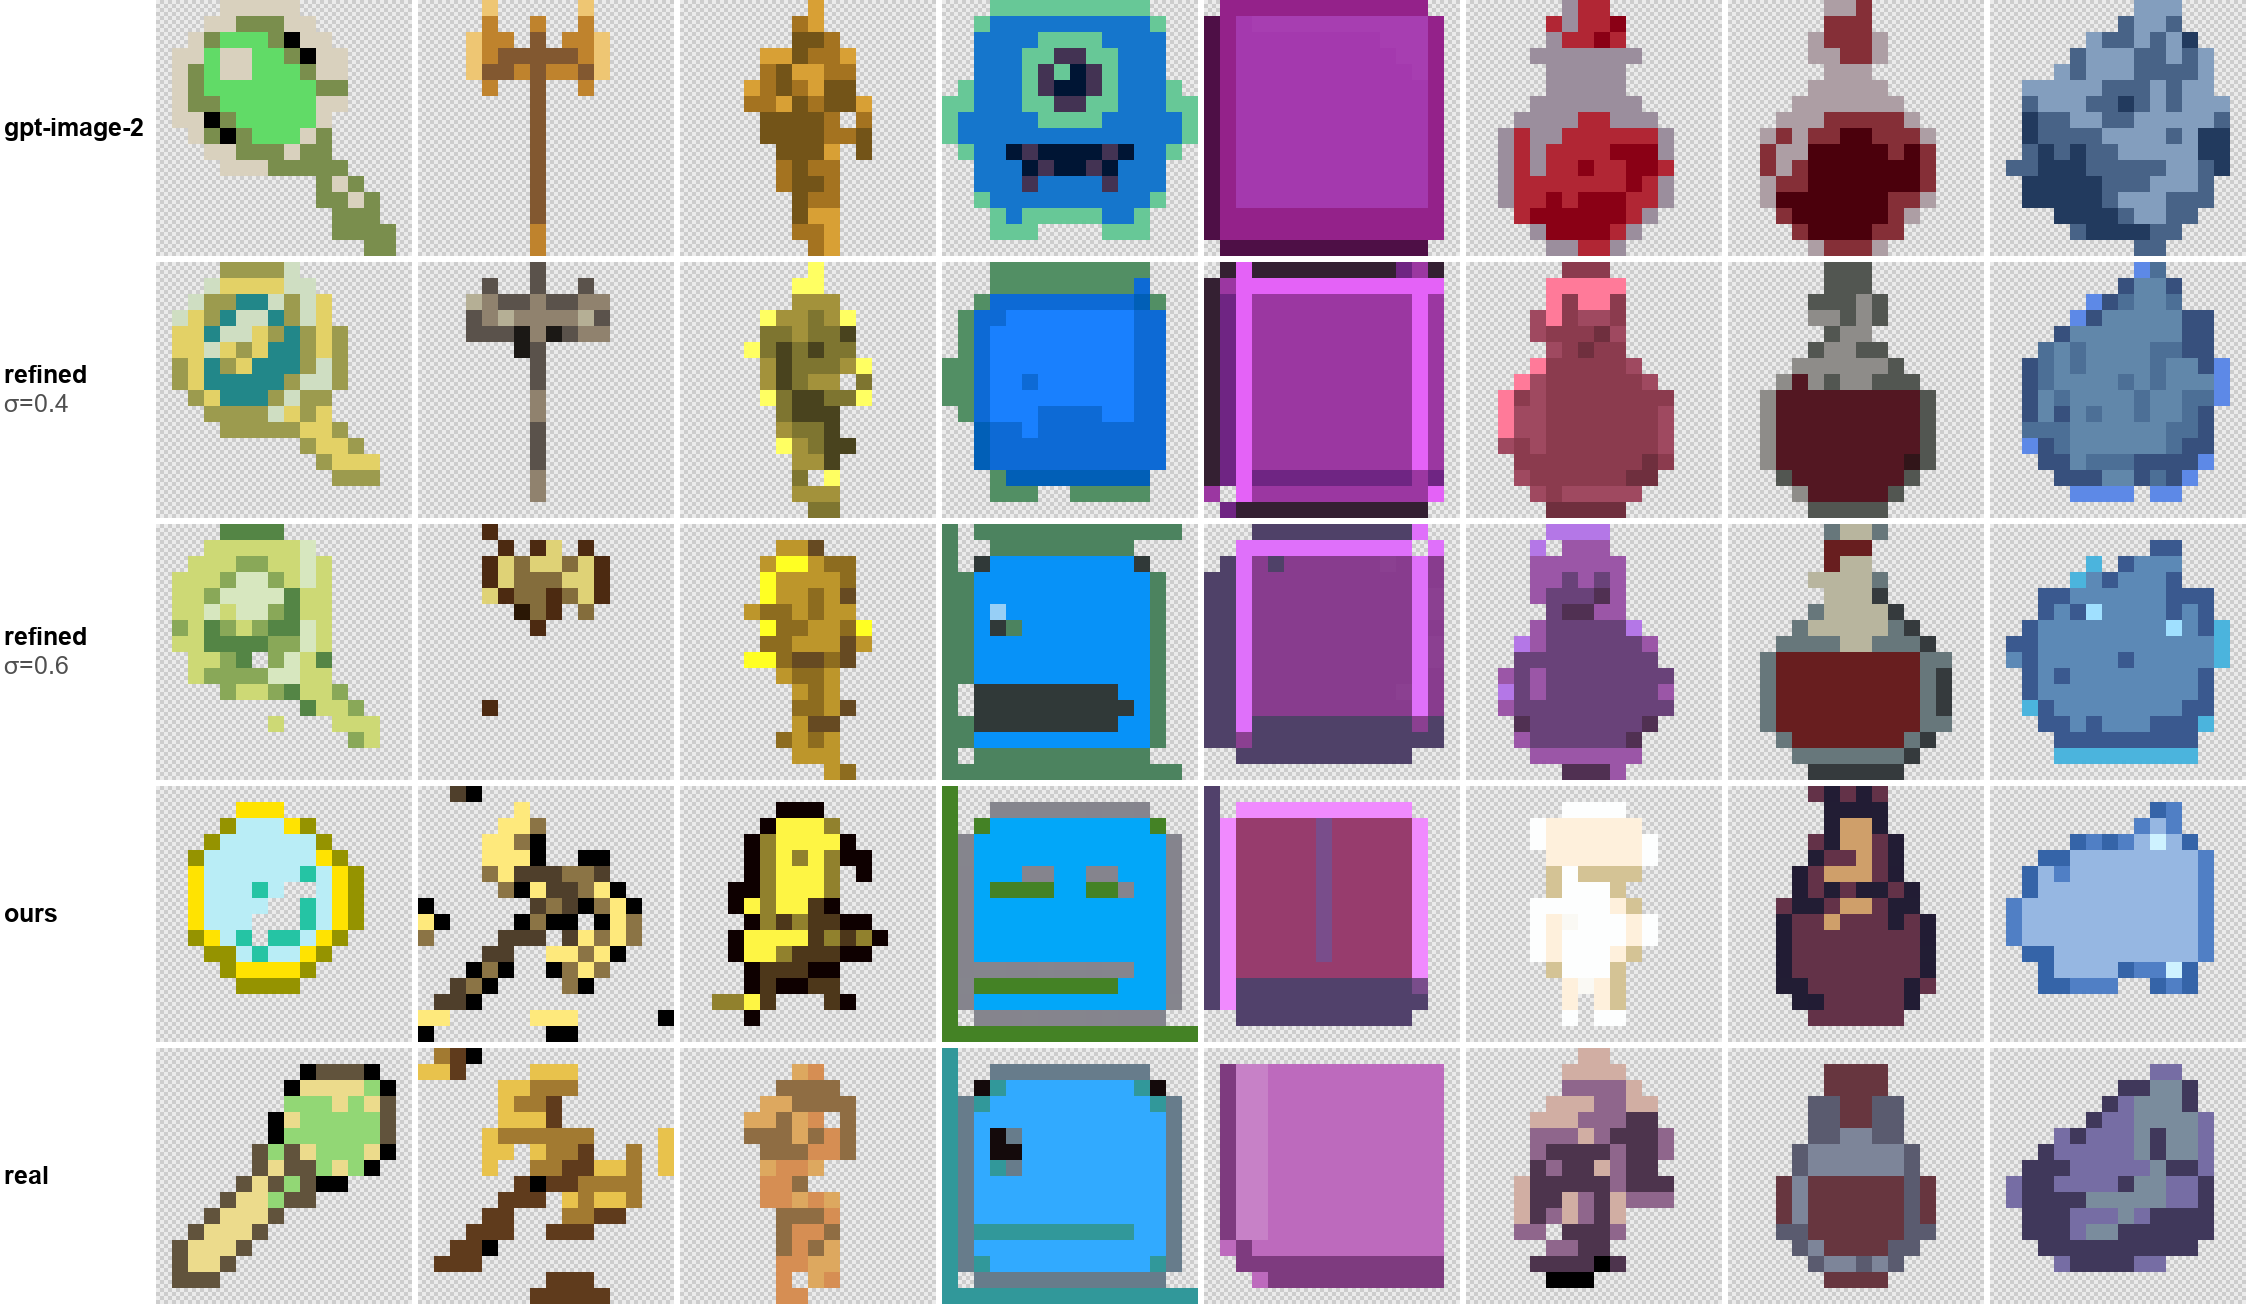
\includegraphics[width=0.72\linewidth]{figures/fig_refine.png}
\caption{Palette Refinement on eight random captions. Rows: gpt-image-2 rendered large and reduced; the same sprite
refined by \ours{} at $\sigma=0.4$ and $\sigma=0.6$; \ours{} generating the caption from noise; the held-out sprite.
Refinement keeps the subject and layout of the input while converting its colours and edges to native pixel art.}
\label{fig:refine}
\end{figure}

\subsection{Analysis}
\label{sec:analysis}

\begin{table}[t]
\centering
\begin{minipage}[t]{0.48\linewidth}
\centering
\caption{Per-image statistics at 16\,px: median opaque colours and fraction of exactly equal adjacent opaque pixels.}
\label{tab:stats}
\small
\begin{tabular}{@{}lcc@{}}
\toprule
& Colours & Flat pairs \\
\midrule
Native reference (real)     & 6  & 0.46 \\
Biased reference            & 34 & 0.20 \\
\midrule
gpt-image-2, reduced        & 93 & 0.01 \\
CFG 1.5                     & 52 & 0.08 \\
ICG $w{=}2$                 & 49 & 0.08 \\
\textbf{\ours{}, $k{=}6$}   & \textbf{6} & \textbf{0.43} \\
\ours{}, $k{=}4$            & 4  & 0.54 \\
\bottomrule
\end{tabular}
\end{minipage}\hfill
\begin{minipage}[t]{0.49\linewidth}
\centering
\caption{Fraction of each set that a provenance probe (logistic regression on DINOv2 features), trained only on real
sprites, calls natively drawn at 16\,px.}
\label{tab:probe}
\small
\begin{tabular}{@{}lc@{}}
\toprule
Set & Native \\
\midrule
\gray{Real held-out sprites (control)}  & \gray{94.9\%} \\
\midrule
gpt-image-2, reduced                    & 4.5\% \\
FLUX.2 + LoRA, palette post-process     & 30.5\% \\
gpt-image-2, palette post-process       & 33.0\% \\
\ours{} w/o PPS                         & 36.8\% \\
\textbf{\ours{}}                        & \textbf{67.5\%} \\
\bottomrule
\end{tabular}
\end{minipage}
\end{table}

\paragraph{PPS reproduces the statistics of the medium.}
Table~\ref{tab:stats} shows why the decoding rule works. Every continuous sampler, as well as gpt-image-2, emits 49--93
colours with almost no exactly flat regions. PPS moves the samples from far outside the medium to inside it: at $k=6$
\ours{} matches the real palette size exactly and reaches 0.43 flat pairs against 0.46 for real sprites.

\paragraph{A provenance probe.}
We fit a logistic
regression on DINOv2 features to separate real sprites drawn at 16\,px from 25--64\,px artwork reduced to 16\,px, using
only real images and holding out the native pool used elsewhere. It reaches 93.0\% held-out accuracy and calls 94.9\% of
unseen real sprites native. The probe shares its features with the FD and responds to palette size and edge hardness,
so we read it as a complementary view of the same property rather than an independent judgement of quality.
Table~\ref{tab:probe} shows that PPS nearly doubles the fraction of our samples classified as natively drawn (36.8\%
$\to$ 67.5\%), while the external systems stay near one third even after quantisation. The same holds at 20\,px (42.4\% $\to$ 58.7\%) and 24\,px (28.1\% $\to$ 42.7\%), and
Palette Refinement at $\sigma=0.6$ raises gpt-image-2 from 33.0\% to 53.0\% and FLUX.2 from 30.5\% to 58.5\%.

\paragraph{Generalisation beyond the training pool.}
The native reference is drawn from the same pool as the training data. To rule out that the gains reflect proximity to
training images, we evaluate on the 210 held-out sprites that are natively $\le 16$\,px and were excluded from training,
using their captions as prompts and the sprites themselves as ground truth; removing every prompt whose sprite has a
near-duplicate in training leaves 124. The ordering is unchanged: \ours{} 61.1, ICG 76.2, CFG 1.5 97.7, against 34.4
for the real sprites themselves (all $n=124$; Appendix~\ref{app:more}), so PPS closes 36\% of the gap between ICG and
real data on sprites the model has never seen. The same holds when prompts with near-duplicate twins are removed from the main evaluation
(below).

\paragraph{The native protocol changes the conclusions.}
The biased reference is a population of blurred illustrations (34 colours, 0.20 flat pairs; Table~\ref{tab:stats}), so
it rewards samplers that produce them. A one-pass sampler that internalises guidance \citep{Chen2025gft} is best under
the biased reference and worst under the native one (Appendix~\ref{app:crossres}); PPS would be discarded by the biased
one.

\paragraph{Robustness of the evaluation.}
Removing the 41.4\% of prompts with a near-duplicate in training changes no ordering (\ours{} 31.8$\to$29.0); an
object-only protocol, Inception-v3 and longer training agree (Appendix~\ref{app:more}).

% ================================================================================================================
\section{Conclusion}
\label{sec:conclusion}

We proposed \ours{} for 12--24\,px sprites at their native resolution. Native-Resolution Target Rebuilding and a
native protocol fix contaminated targets; Palette-Projected Sampling enforces a per-sprite palette inside the sampler
and, with SDEdit-style re-noising, refines external sprites.
\emph{Limitations.} A VLM judge prefers polished renders over real sprites
(Appendix~\ref{app:more}), so a human study is the natural next step; PPS at $k=4$ trades a little retrieval for
fidelity ($k=6$ matches real sprites).

% ================================================================================================================
\section*{Reproducibility statement}
Section~\ref{sec:model} and Appendix~\ref{app:details} specify the architecture, training recipe and sampler, and
Eq.~(\ref{eq:palette}) with Section~\ref{sec:palette} fully specifies Palette-Projected Sampling. Section~\ref{sec:data}
and Appendix~\ref{app:data} give every step of the data rebuild with per-step counts. Section~\ref{sec:protocol} and
Appendix~\ref{app:details} specify the evaluation protocol: prompt set, chunked seeding, reference sets, preprocessing
and floors. Section~\ref{sec:external} and Appendix~\ref{app:externalfig} describe the conversion pipelines for the
external systems, and Appendix~\ref{app:crossres} the cross-resolution samplers. We will release code for
training, sampling, palette projection and evaluation, the captions, the per-sprite licence manifest of the new
material and the held-out split.

\section*{Ethics statement}
The model generates small game sprites. It adds no capability beyond existing text-to-image systems, and its outputs
(12--24\,px) have little potential for targeted misuse. Its intended application raises the usual concerns of generative
art tools, namely the displacement of pixel artists and the reproduction of styles present in the training corpus. The
training data are community sprites from OpenGameArt and the Kenney and Liberated Pixel Cup packs. The 14{,}999 sprites
added in this work carry a recorded source zip, member path and licence (CC-BY-4.0, CC-BY-SA-3.0, OGA-BY-3.0); the older
material predates that bookkeeping, so a per-asset licence audit precedes any release of the full corpus. Captions were
produced by a commercial vision--language model; external baselines were generated through commercial APIs under their
terms of use. No human subjects were involved.

\section*{AI use statement}
% Required by ICLR 2027 (does not count toward the page limit). The authors must complete and confirm this section.
Generative AI tools were used in this work in the following ways. (a) Inside the method and its data pipeline:
vision--language models produced the training and evaluation captions (gemini-3-flash \citep{Gemini3} for the original corpus,
gemini-3.8-flash for the material added here), labelled every evaluation sprite by content type and rated sprite craft
for the ablations of Appendix~\ref{app:more}; commercial image generators served as external baselines
(Section~\ref{sec:external}). Each of these uses is an experimental component, is described where it is used, and its
outputs were spot-checked against manual inspection --- the caption classifier was validated against image-level labels
on 2{,}980 held-out sprites (82.5\% agreement), and the content and craft labels were checked on random grids by the
authors. (b) In the research process: an LLM-based coding assistant implemented and ran experiments, searched and
verified related work, and drafted and edited parts of this manuscript. Every number reported here comes from a script
in the released code and was regenerated from the saved samples; the authors reviewed all AI-assisted work and take
responsibility for the final content, its claims and its errors.

\bibliography{refs}
\bibliographystyle{iclr2027_conference}

\appendix
% Appendix of the ICLR 2027 draft (input from main.tex after the bibliography).

\section{The rebuilt corpus, step by step}
\label{app:data}

\paragraph{Counts.}
The original corpus holds 37{,}489 unique sprites (after cutting sheets into connected components at native scale and
dropping glyphs, UI and near-monochrome crops). Native sizes: 710 at most 12\,px, 2{,}675 at most 16\,px, 9{,}687 at
most 20\,px, 12{,}516 at most 24\,px, 19{,}611 at most 32\,px. Exact-pixel hashing finds 4{,}888 duplicate copies;
16.2\% of the 3{,}000 held-out evaluation sprites and 17.0\% of the 200 external-comparison sprites have a
pixel-identical twin that the path-based hold-out leaves in training. Integer-upscaled pixel art, which could be
restored by dividing by its block size, accounts for only 4.6\% of the corpus.

\paragraph{New material.}
The CC-BY-4.0, CC-BY-SA-3.0 and OGA-BY-3.0 OpenGameArt collections (8.8\,GB of 2D art) yield 37{,}226 cut sprites.
Filtering by the same rules removes 8{,}184; cross-corpus pixel hashing removes a further 6{,}062 that duplicate the
existing corpus; a filename filter removes 367 font, UI and text sheets; average-hash collapse of animation frames
removes 3{,}456; a cap of 60 sprites per source sheet removes the rest, leaving 14{,}999 sprites from 1{,}207 sheets.
Verification of this set: median palette 6 colours, 98.2\% of visible pixels fully opaque, mean flat-neighbour fraction
0.434, native sizes 234 / 1{,}726 / 5{,}374 / 6{,}028 at most 12 / 16 / 20 / 24\,px. Every sprite keeps its source zip,
member path and licence in a manifest.

\paragraph{Captions.}
We caption the new sprites with gemini-3.8-flash on numbered $4\times5$ grids of nearest-upscaled sprites on a
checkerboard, one caption per cell, 6--15 words, with an explicit ``unclear abstract shape'' escape. Of 14{,}999
sprites, 14{,}845 receive a caption (99.0\%); dropping the escapes, degenerate strings and 11 rows that echoed the
instruction leaves 13{,}987 usable captions, 99.6\% distinct, median 13 words. We selected the captioner by running the
same grid through ten vision--language models: gemini-3.8-flash parsed all 20 cells in both trials at 22\,s per call and
was the most accurate, while a larger sibling truncated at cell 11 in both trials and several models mislabelled
weapons and buildings.

\paragraph{Training-set composition.}
With duplicates removed and downscaling limited to $1.5\times$, the rebuilt corpus yields 86{,}290 training rows
(12/16/20/24\,px buckets: 7{,}357 / 11{,}733 / 15{,}087 / 17{,}199), against 64{,}990 without the new sprites and
180{,}533 under the original policy, which fed 48\,px artwork to the 16\,px bucket.

\paragraph{Near-duplicate collapse is harmful.}
Collapsing average-hash near-duplicates in the \emph{old} corpus as well (37{,}489 $\to$ 26{,}504 groups) costs more
than it gains: at 20k steps it scores 21.07 biased / 162.23 native against 20.31 / 151.85 for the same recipe without
the collapse. We therefore drop only exact duplicates in the main corpus and apply the collapse only to the new
material, where single sheets contributed up to 563 frames of one character.

\section{Cross-resolution guidance: equations and full tables}
\label{app:crossres}

The cross-resolution rules referenced in Section~\ref{sec:analysis} use the guided prediction
$\tilde e = \eref + w\,(e_{\text{strong}} - \eref)$ with
\begin{equation}
  \eref^{\text{label}} = \epsilon_\theta(x_t, t, c, \blow), \qquad
  \eref^{\text{comp}} = \epsilon_{\theta_{\text{snap}}}(x_t, t, c, \blow), \qquad \blow < b_R,
  \label{eq:ref}
\end{equation}
i.e.\ the same network (or an early EMA snapshot of it) queried under a lower resolution bucket, with $\blow = 12$ at
16\,px and $\blow = 16$ at 20 and 24\,px. The internalised variant follows guidance-free training \citep{Chen2025gft}:
the network gains a scalar input $\beta \in (0,1]$ and is trained with
\begin{equation}
  \hat\epsilon_\beta(x_t, t, c, b) = \beta\,s_\theta(x_t, t, c, b, \beta) + (1-\beta)\,\sg[\epsilon_{\theta_{\text{snap}}}(x_t, t, c, \blow(b))],
  \label{eq:gft}
\end{equation}
so that setting $\beta = 1/w$ at inference reproduces the rule of Eq.~(\ref{eq:ref}) in a single forward pass. The
internalised model is initialised from the base model and trained for 10k further steps (Table~\ref{tab:hparams}).

On the rebuilt model, scored against native pixel art, these rules give 114.9 (label), 117.0 (composed), 178.8
(internalised, $\beta = 1$) and 170.3 (internalised, $w = 1.5$), against 113.2 for CFG 1.0 and 87.1 for ICG; under the
biased reference the internalised model is the best row of Table~\ref{tab:full16} (10.4). The reference is a
lower-resolution belief, so extrapolating away from it adds contrast without reducing the palette, which the biased
reference rewards and the native one does not.

\section{Implementation and protocol details}
\label{app:details}

\begin{table}[h]
\caption{Training and sampling configuration.}
\label{tab:hparams}
\centering
\small
\begin{adjustbox}{max width=\linewidth}
\begin{tabular}{@{}ll@{}}
\toprule
Denoiser & diffusers \texttt{UNet2DConditionModel}, 4 input/output channels (RGBA), widths 128/256/512, \\
 & 2 layers per block; down: CrossAttn, CrossAttn, plain; up: plain, CrossAttn, CrossAttn; 72.5M parameters \\
Text & frozen CLIP ViT-B/32 text encoder, 77 tokens, last hidden states (512-d) as cross-attention context \\
Resolution & class embedding over $\mathcal{B} = \{12,16,20,24,32,48,64\}$ added to the timestep embedding; never dropped \\
Diffusion & $\epsilon$-prediction, $T = 1000$, cosine (\texttt{squaredcos\_cap\_v2}) schedule \\
Base training & from scratch, 80k steps, AdamW, constant lr $5\cdot10^{-5}$, EMA 0.999, caption dropout 10\% \\
Batches & one bucket per batch, bucket drawn proportionally to its row count; batch 320 / 256 / 224 / 192 / 128 / 64 / 40 \\
 & for 12 / 16 / 20 / 24 / 32 / 48 / 64\,px \\
Sampler & ICG $w{=}2$; PPS with $f{=}0.5$, $k{=}8/4/8/6/8$ at 12/16/20/24/32\,px, 8 $k$-means iterations; opaque = $\hat\alpha > 0.5$ \\
Snapshot & 10k-step EMA of an independent 10k-step run with the same recipe (cross-resolution composed reference only) \\
Internalization & init from the base model, 10k steps, same optimizer/lr/EMA/batches; $\beta\sim\mathcal U(0.4,1)$, $\beta{=}1$ w.p.\ 0.25 and for 12\,px rows; \\
 & reference rung 12 (for 16\,px rows) and 16 (for 20 and 24\,px rows); $\beta$ via 256-d sinusoidal embedding of $1000\beta$ \\
 & and a zero-initialized linear map into the timestep features (32,768 parameters) \\
Sampling & 100-step ancestral DDPM, EMA weights, one sample per prompt \\
\bottomrule
\end{tabular}
\end{adjustbox}
\end{table}

\paragraph{Canvas preprocessing.} A sprite larger than the target side $R$ is reduced with a premultiplied-alpha box
filter, preserving aspect ratio; a sprite at most $R/2$ is enlarged by an integer nearest-neighbour factor. It is then
centred on a transparent $R\times R$ canvas, and alpha is thresholded at 128 (pixels below become fully transparent,
with RGB cleared). Generated samples are stored with the same hard alpha. The same function produces the FD reference
set, the held-out floor set and the ``downscale'' external baselines.

\paragraph{Evaluation prompts and training exclusion.} All real sprites of the original corpus are split once with a
fixed shuffle into a 3,000-sprite \emph{biased} reference set and a disjoint held-out pool. The first 3,000 held-out
sprites supply, through their recaptions, the 3,000 evaluation prompts. The biased reference and these 3,000 held-out
sprites (5,928 paths) are removed from training, together with every exact duplicate of them.

\paragraph{Native reference.} The sprites of the original corpus that are natively at most $R$\,px are split in half with
a fixed seed into the native reference and a disjoint floor set (16\,px: 1,337 and 1,338). This pool is not removed from
training except where it overlaps the 5,928 excluded paths; the training-excluded native set of
Section~\ref{sec:analysis} consists of the floor-set sprites that are among the excluded paths (210 at 16\,px).

\paragraph{FD.} Each image is composited on white and resized to $R\times R$ (box filter; generated images are already
$R\times R$). It is then nearest-neighbour upsampled to $224\times224$, normalized with ImageNet statistics, and embedded
by the CLS token of \texttt{facebook/dinov2-small}. FD is the Fréchet distance between Gaussian fits of the two feature
sets (at 16\,px: 3,000 samples vs.\ 1,337 native or 3,000 biased reference images; 200 samples for the external
comparison). Samples are generated in chunks of 1,000 prompts, and chunk $i$ uses seed $s + i$.

\paragraph{CLIP.} The same saved samples are composited on mid-grey, nearest-neighbour upsampled to 224\,px and scored
with CLIP ViT-B/32 against the caption they were sampled from. We report $100\cos$ and R@1, the fraction of samples
whose own caption ranks first among itself and 99 random held-out captions (chance 1\%).

\section{Recaptioning}
\label{app:recap}

\begin{table}[h]
\caption{Caption statistics before and after recaptioning (43,342 unique training and evaluation images).}
\label{tab:recap}
\centering
\small
\begin{adjustbox}{max width=\linewidth}
\begin{tabular}{@{}lcc@{}}
\toprule
 & BLIP \citep{Li2022blip} (original) & gemini-3-flash \citep{Gemini3} (recaptioned) \\
\midrule
Distinct captions & 23.5\% & 98.6\% \\
Words per caption (median / mean) & 8 / 7.6 & 12 / 12.1 \\
Occurrences of the most frequent caption & 7,669 (``a pixel art sprite'') & 6 (``human'') \\
Share of data covered by the ten most frequent captions & $\approx$25\% & $<$0.1\% \\
\bottomrule
\end{tabular}
\end{adjustbox}
\end{table}

Images were sent as numbered grids on a checkerboard (20 per request, 12 for retries). For each cell, the instruction
asked for a caption of 6--15 words that names the object first and then its distinguishing colours, materials and
parts, describes only what is visible, and avoids uninformative words (``pixel art'', ``sprite'', ``8-bit'', ``icon'').
Of the 43,342 unique images, 41,560 received a caption and 41,103 (94.8\%) were usable. The remainder were declared an
``unclear abstract shape'' by the captioner and keep their BLIP \citep{Li2022blip} caption. Across the three caption files (49,652 rows),
95\% of rows were replaced. The total cost was about 18.7M tokens. The held-out evaluation prompts are the recaptions of
the held-out sprites, so the evaluation prompts follow the training caption distribution.

\section{External systems: pipeline and qualitative comparison}
\label{app:externalfig}

The gpt-image-2 \citep{GPTImage2} renders were requested at 1024\,px through the vendor's image-generation API with the
prompt ``\emph{<recaption>}, pixel art sprite of a single object, plain flat white background, centred, no text''. The
sprite is cut out by flood-filling, from the image border, all pixels within 18 (per channel, 8-bit) of the median border
colour, and then cropped to its content. \emph{Downscale} applies our canvas preprocessing (Appendix~\ref{app:details}).
\emph{PixelOE} pads the cut-out to a square on white, pixelizes the RGB in contrast mode with colour matching directly to
$R\times R$, and takes alpha by majority vote of the cut-out mask in each cell. \emph{Make Your Own Sprites} resizes the
same square to $4R\times4R$ (bicubic), applies the official network with 4\,px cells, and reduces the output by 4 with
nearest-neighbour sampling, with alpha as for PixelOE. We bypass the official script's minimum input size of 128\,px,
because it would change the cell count for 12--24\,px targets. The SDXL + Pixel Art XL LoRA row uses SDXL base 1.0 with
the fused LoRA (scale 1), Euler with 30 steps, CFG 7 and the same prompt and conversions.

\paragraph{Choice of conversion.} We compared the three conversions on gpt-image-2 renders of the 200 captions against
the corpus-sample reference, without palette post-process: box downscaling gives 82.2 at 16\,px, PixelOE 146.3 and
Make Your Own Sprites 155.2 (20\,px: 317.6 / 282.5 / 336.7; 24\,px: 428.5 / 358.0 / 431.2). Box downscaling is best at
16\,px, where the main comparison is made, and we use it for every external system at every resolution.

\section{Captions of the qualitative figures}
\label{app:prompts}

Held-out prompt indices 3, 7, 12, 20, 33, 41, 55, 67, left to right in Figure~\ref{fig:external}:
\begin{enumerate}[leftmargin=1.6em,itemsep=0pt]
  \item Crou \emph{(a caption the vision model could not resolve; kept to show the untouched prompt distribution)}
  \item Alien soldier, blue with green armor, lunging forward while gripping a black rifle
  \item Top-down character head with brown hair, black goggles, white antenna, and pale skin
  \item Platypus like creature with brown body, yellow beak, and large eyes in swimming pose
  \item Man: blocky person with short brown hair, red shirt, and dark blue pants
  \item Stone brick wall with yellow rectangular bricks and a central red gem
  \item Large fire, white-yellow core, intense orange glow, dark red jagged outlines
  \item Glowing sun, bright yellow center with an orange border and a white cross
\end{enumerate}

Figure~\ref{fig:palette} uses indices 11, 20, 33, 50, 67 of the same file.

\section{Additional analyses}
\label{app:more}

\paragraph{Full 16\,px table with both references.}
Table~\ref{tab:full16} lists every 16\,px configuration under the native and the biased reference. The two columns rank
samplers in opposite orders, which is the effect analysed in Section~\ref{sec:analysis}.

\begin{table}[h]
\caption{16\,px, 3{,}000 held-out captions. \emph{Native}: reference drawn only from sprites natively $\le 16$\,px
(floor 4.47). \emph{Biased}: a random corpus sample (floor 3.45), 92.9\% of which is downscaled artwork.}
\label{tab:full16}
\centering
\small
\begin{tabular}{@{}llcc@{}}
\toprule
Targets & Sampler & Native FD $\downarrow$ & Biased FD \\
\midrule
original                 & CFG 1.5                            & 167.2 & 11.1 \\
w/o new sprites          & CFG 1.5                            & 123.1 & 14.8 \\
rebuilt                  & CFG 1.0 / 1.5 / 2                  & 113.2 / 117.9 / 131.1 & 19.0 / 13.6 / 12.2 \\
rebuilt                  & cross-resolution label reference, $w{=}1.5$ & 114.9 & 14.2 \\
rebuilt                  & composed reference, $w{=}1.5$      & 117.0 & 12.8 \\
rebuilt                  & internalised (1 \nfe), $w{=}1.5$   & 170.3 & 10.4 \\
rebuilt                  & ICG $w{=}1.5$ / $2$                & 87.2 / 87.1 & 16.2 / 20.7 \\
rebuilt                  & ICG $w{=}1.5$ + post-hoc 4 colours & 41.6 & 111.0 \\
rebuilt                  & ICG $w{=}1.5$ + PPS $k{=}4$        & 34.1 & 111.0 \\
rebuilt                  & ICG $w{=}2$ + PPS $k{=}6$          & 36.9 & 71.1 \\
rebuilt                  & ICG $w{=}2$ + PPS $k{=}4$          & 31.8 \pmsd{0.49} & 111.2 \\
\bottomrule
\end{tabular}
\end{table}

\paragraph{Palette size per resolution.}
Native FD with ICG $w{=}2$ for each palette size: at 12\,px 143.2 ($k{=}8$), 143.3 ($k{=}6$), 145.2 ($k{=}10$), 150.7
($k{=}5$), 156.5 ($k{=}4$); at 20\,px 96.5 ($k{=}8$), 99.1 ($k{=}6$), 110.7 ($k{=}4$); at 24\,px 123.6 ($k{=}6$), 128.4
($k{=}4$), 130.1 ($k{=}8$); at 32\,px 74.5 ($k{=}8$), 78.7 ($k{=}12$). Drawing $k$ per sprite from the corpus histogram
gives 39.9 at 16\,px.

\paragraph{Native ground truth.}
A second evaluation set uses as ground truth the 210 held-out sprites that are natively $\le 16$\,px and were excluded
from training (124 after removing prompts whose sprite has a near-duplicate twin in training;
Figure~\ref{fig:nativegt}). On the 124 prompts the ordering is the same as in Table~\ref{tab:main16}: CFG 1.5 97.7,
ICG $w{=}2$ 76.2, \ours{} 61.1; the real sprites themselves score 34.4, which is the reference point of this set.

\begin{figure}[h]
\centering
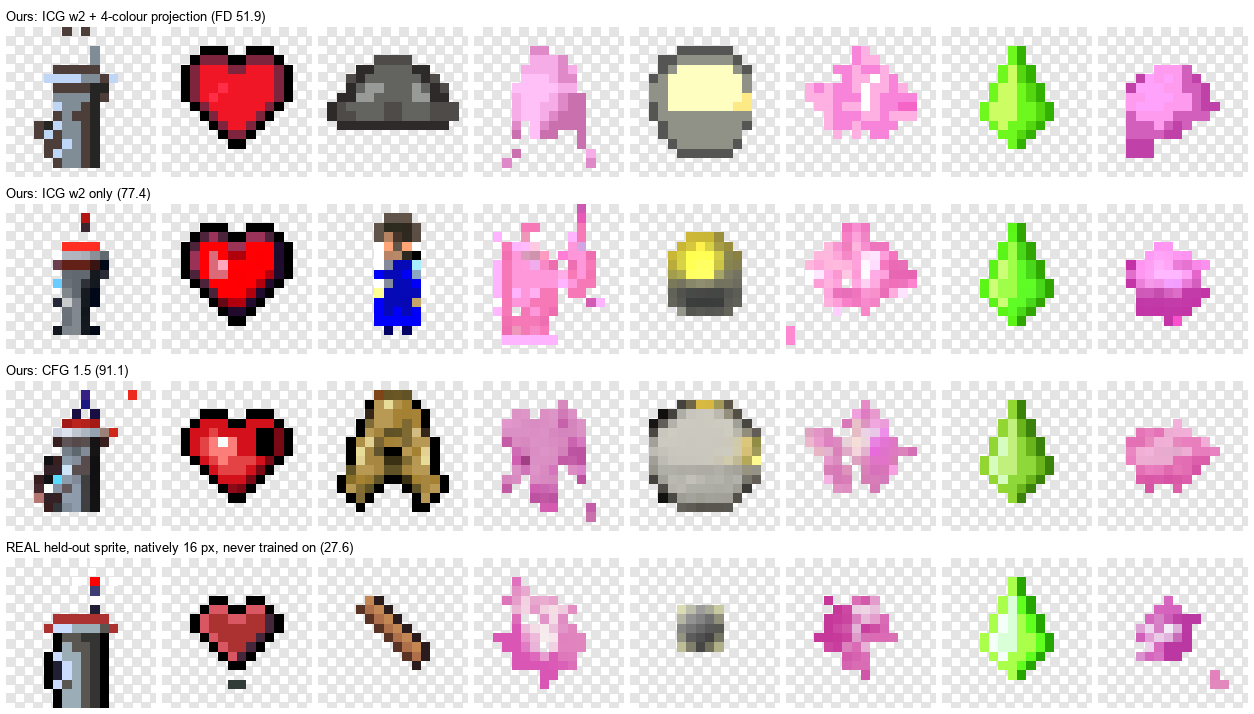
\includegraphics[width=\linewidth]{figures/fig_native_gt.png}
\caption{Twelve prompts from the training-excluded native set (sprites drawn at 16\,px and removed from training).
Rows: \ours{}; ICG only; FLUX.2-klein with a pixel-art LoRA, downscaled; the real sprite. Numbers in the row titles are
native FD on all 210 prompts of this set, including those with near-duplicate twins in training; the text reports the
124-prompt subset without them.}
\label{fig:nativegt}
\end{figure}

\paragraph{Robustness of the evaluation.}
\emph{Near-duplicate leakage}: removing the 41.4\% of prompts whose sprite has a near-duplicate twin in training
($8\times8$ average hash) changes every number by at most 3.0 FD and no ordering (\ours{}: 31.8 $\to$ 29.0).
\emph{Content}: restricting both reference and prompts to sprites a vision--language model labels as standalone objects
gives 37.1 for \ours{} against 103.0 for ICG and 144.9 for CFG (see Content labels below). \emph{Feature space}:
Inception-v3 clean-FID preserves the ordering with smaller margins (below). \emph{Training length}: 100k and 120k steps
give 30.8 and 32.3, so the model is converged.

\paragraph{Inception features.}
Inception-v3 clean-FID \citep{Parmar2022} and KID \citep{Binkowski2018} on the same saved samples and native reference preserve the ordering:
PPS $k{=}4$ 23.79, $k{=}6$ 23.28, no projection 26.27, CFG 29.37, one corpus-wide palette 36.05, median filter 66.63
(real held-out 10.54). The separation is smaller than under DINOv2 because Inception resizes its input to 299\,px,
which blurs the hard edges and flat interiors that distinguish 16\,px pixel art.

\paragraph{Content labels.}
A vision--language model labels every evaluation image (20 per numbered grid; classes object, effect, fragment, glyph,
junk). Of the 3{,}000 held-out sprites, 73.2\% are standalone objects, 15.7\% fragments, 7.8\% effects, 2.0\% glyphs and
1.3\% junk. The object-only protocol of Section~\ref{sec:analysis} keeps 825 reference sprites and 2{,}181 prompts
(\ours{} 37.1, ICG 103.0, CFG 144.9, original targets 201.3, real mixed-provenance sprites 161.3). Dropping the 8{,}818
sprites labelled fragment, glyph or junk from training improves a 20k-step run from 165.6 to 156.7 native FD; we keep
the unfiltered corpus for simplicity.

\paragraph{Training length, capacity and data scale.}
The headline model is converged: 31.8, 30.8 and 32.3 native FD at 80k, 100k and 120k steps. A $2.2\times$ larger UNet
(161.2M parameters) reaches 38.5 at 80k, so the 72.5M model is the better choice at this data scale. Adding the Kenney
CC0 packs and the OpenGameArt CC-BY-3.0 bundle (118{,}378 training rows) improves a 20k-step run from 54.2 to 42.9 but
gives $39.3\pm0.3$ at 80k against $31.8\pm0.5$ for the main corpus. Because both the capacity and the data-scale
comparisons reorder between 20k and 80k steps, every headline number in this paper is measured at full training length.
Replacing CLIP ViT-B/32 with ViT-L/14 as the text encoder gives 164.0 against 165.6 at 20k steps.

\paragraph{Quality conditioning.}
A vision--language model rates each sprite's craft from 1 to 5, and we train a separate model with the rating prepended
to the caption as a tag. Asking for the top tag at sampling time produces visibly more finished sprites
(Figure~\ref{fig:qualtag}). Because the tag concentrates the output on the best-rated 8\% of the corpus, which is
dominated by items and characters, distributional scores against the full native reference increase: the tag-trained
model scores 45.6 with the top tag and 34.2 without it, against 31.8 for the main model. We therefore keep the main model
unconditioned and offer the tag as a practitioner's control.

\begin{figure}[h]
\centering
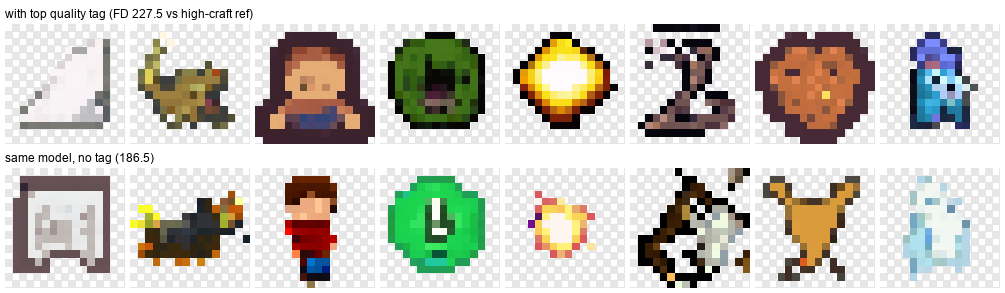
\includegraphics[width=\linewidth]{figures/fig_quality_tag.png}
\caption{Quality conditioning at 16\,px: same model, prompts and seed, sampled with (top) and without (bottom) the top
craft tag.}
\label{fig:qualtag}
\end{figure}

\paragraph{Vision--language model as a judge.}
We also put 560 forced-choice pairs over 40 captions to a vision--language model, with real held-out sprites in the pool
as a control. \ours{} ties with the real sprites (50\%) under two different question wordings. The judge, however, also
prefers the polished renders of FLUX.2 and gpt-image-2 over real sprites (72\% and 70\%), which indicates that a
general-purpose vision model responds to polish rather than to whether an image was authored at sprite resolution; this
is the property the native reference set is designed to capture, and it is why we do not use such a judge as a
substitute for a human study.

\paragraph{Canvas occupancy.}
Real sprites drawn at 16\,px cover 26\% of their canvas, while sprites that are resized to fill a bucket cover about
40\%; \ours{} covers 34\%. Preserving each sprite's native margin during bucketing is a simple extension that we leave to
future work.


\end{document}
